% Generated by code/scripts/report_figures.py at 2026-11-16T12:31:35Z; do not edit.
% Inputs: artifacts/cluster/runs/bench1-20261107T033925Z-1528774
\begin{figure}[t]
\centering
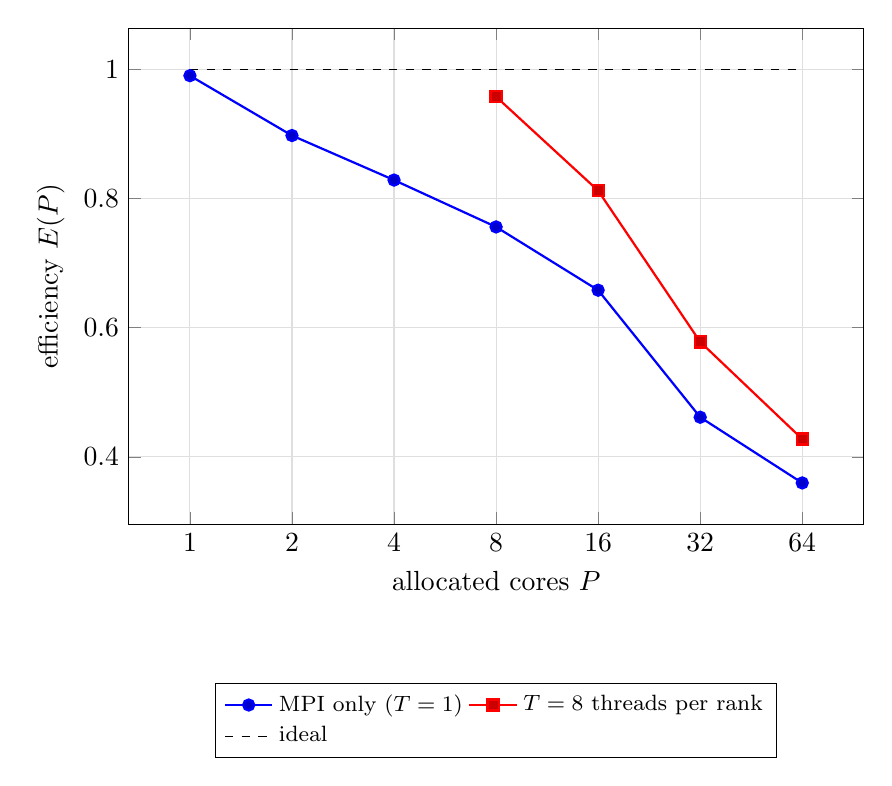
\begin{tikzpicture}
\begin{axis}[width=0.9\columnwidth, height=0.65\columnwidth, xlabel={allocated cores $P$}, ylabel={efficiency $E(P)$}, xmode=log, log basis x=2, log ticks with fixed point, legend style={at={(0.5,-0.32)}, anchor=north, legend columns=2, font=\footnotesize}, legend cell align=left, grid=major, grid style={gray!25}]
\addplot+[mark=*, thick] coordinates {(1,0.9905) (2,0.8978) (4,0.8288) (8,0.7562) (16,0.6582) (32,0.4614) (64,0.3596)};
\addlegendentry{MPI only ($T=1$)}
\addplot+[mark=square*, thick] coordinates {(8,0.9579) (16,0.8124) (32,0.5781) (64,0.4276)};
\addlegendentry{$T=8$ threads per rank}
\addplot[black, dashed] coordinates {(1,1) (64,1)};
\addlegendentry{ideal}
\end{axis}
\end{tikzpicture}
\caption{Strong-scaling efficiency. $N=10^{6}$, median of repetitions; serial Barnes--Hut baseline on the same CPU model and build. Vanda job 1528774: all 64 cores of Gold 6438N node IN-008, 3 interleaved repetitions.}
\label{fig:strong-efficiency}
\end{figure}
